\section{Метрики}
\label{sec:Metrics} \index{Metrics}

\subsection{ASR}
\hspace{0.6cm}Метрика \textbf{ASR (Attack Success Rate)} характериузет процент успешных атак на модель. Под атакой подразумевается подача в модель состязательного и исходного текстов и дальнейшее исследование выходов. Атака считается успешной, если прогноз модели изменился (в случае классификации текстов: произошла смена предсказанного класса), то есть ASR метрика показывает, на каком проценте текстов исходная модель изменила свой прогноз. Таким образом, чем выше ASR, тем лучше оказался метод генерации состязательного примера. ASR можно записать следующей формулой:

\begin{equation*}
    ASR = \left( \frac{\text{Число успешных атак}}{\text{Общее число атак}} \right) \times 100
\end{equation*}


\subsection{USE}
\hspace{0.6cm}На высоком уровне идея метрики \textbf{USE (Universal sentence encoder)} состоит в том, чтобы разработать кодировщик, который для любого заданного предложения извлекает N-мерное векторное представление (для BERT-подобных моделей N чаще всего равно 512). Данный кодировщик представляет из себя суммаризатор, который на любую ограниченную по длине последовательность токенов выдаёт числовой вектор данной последовательности. Используя данные вектора и косинусную метрику, можно оценивать схожесть двух и более текстов между собой: 1-значит они семантически индентичны, -1-значит тексты совсем не похожи друг на друга. Аналогично ASR чем выше метрика USE, тем лучше, так как важно наравне с успешностью атаки сохранить исходный семантический смысл текста. Существует несколько вариантов кодировщика для вычисления вектора предложения:

\subsubsection{\textbf{Кодировщик трансформера (BERT)}}
\hspace{0.6cm}В этом варианте используется энкодерная часть оригинальной архитектуры трансформера. Архитектура состоит из 2-24 многоуровневых слоев. Каждый слой включает в себя \textbf{механизм внимания}, за которым следует последовательность \textbf{полносвязных слоёв} и \textbf{нормализация} по каждому отдельному латентному вектору. На выходе получается 768-мерный вектор в качестве векторного представления входного предложения.

\subsubsection{\textbf{Deep Averaging Network (DAN-кодировщик)}}
\begin{wrapfigure}{l}{0.5\textwidth}
    \centering
    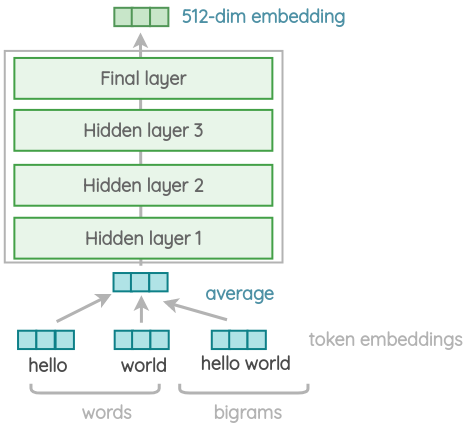
\includegraphics[width=1\linewidth, height=8.5cm]{pictures/dan.png}
    \caption{Архитектура DAN}
    \label{fig:Архитектура DAN}
\end{wrapfigure}
\hspace{0.6cm}В этом варианте кодировщик представляет из себя последовательность подряд идущих \textbf{fully-connected слоёв} нейронной сети. Векторное представление слов и биграмм, присутствующие в предложении, усредняются вместе. Затем они проходят через n-слойный глубокий DNN с прямой связью, чтобы получить 512-мерный вектор предложения в качестве выходных данных.